\documentclass[12pt]{scrartcl}

\usepackage[
  a4paper, mag=1000,
  left=2cm, right=1cm, top=2cm, bottom=2cm, headsep=0.7cm, footskip=1.27cm
]{geometry}

\usepackage[T2A]{fontenc}
\usepackage[utf8]{inputenc}
\usepackage[english,russian]{babel}
\usepackage{cmap}
\usepackage{amsmath}
\usepackage{tabularx}
\usepackage{graphicx}
\usepackage{array}
\IfFileExists{pscyr.sty}{\usepackage{pscyr}}{}
\usepackage[parfill]{parskip}
\usepackage{lastpage}
\usepackage{setspace} % single spacing between lines
\usepackage{blindtext} % for generated text - can remove
\usepackage{titlesec} % set header spacing
\setlength{\parindent}{15pt} % paragraph indent

\titlespacing{\section}{0pt}{\parskip}{-\parskip}
\titlespacing{\subsection}{0pt}{\parskip}{-\parskip}
\titlespacing{\subsubsection}{0pt}{\parskip}{-\parskip}

\usepackage[numbered]{bookmark}
\clubpenalty=10000
\widowpenalty=10000

\usepackage{fancybox,fancyhdr}
\pagestyle{fancy}
\fancyhf{}
\fancyhead[C]{\small{Олимпиадное программирование (средний уровень). Тренировка 03 \\ Летняя компьютерная школа ``КЭШ'', 6--26 августа 2016 года}}

%user-defined commands

\newcommand{\inputFile}{Стандартный ввод}
\newcommand{\outputFile}{Стандартный вывод}

\begin{document}

\singlespacing

\section*{Задача A. 12 месяцев}

\begin{tabularx}{\textwidth}{l l X}
    Имя входного файла: & \texttt{\inputFile} \\
    Имя выходного файла: & \texttt{\outputFile} \\
    Ограничение по времени: & $2$ секунды \\
    Ограничение по памяти: & $256$ мегабайт \\
    Автор: & \emph{Павел Атнашев~---~USU Championship 2004} 
\end{tabularx}

\begin{figure}[h]
	\centering
    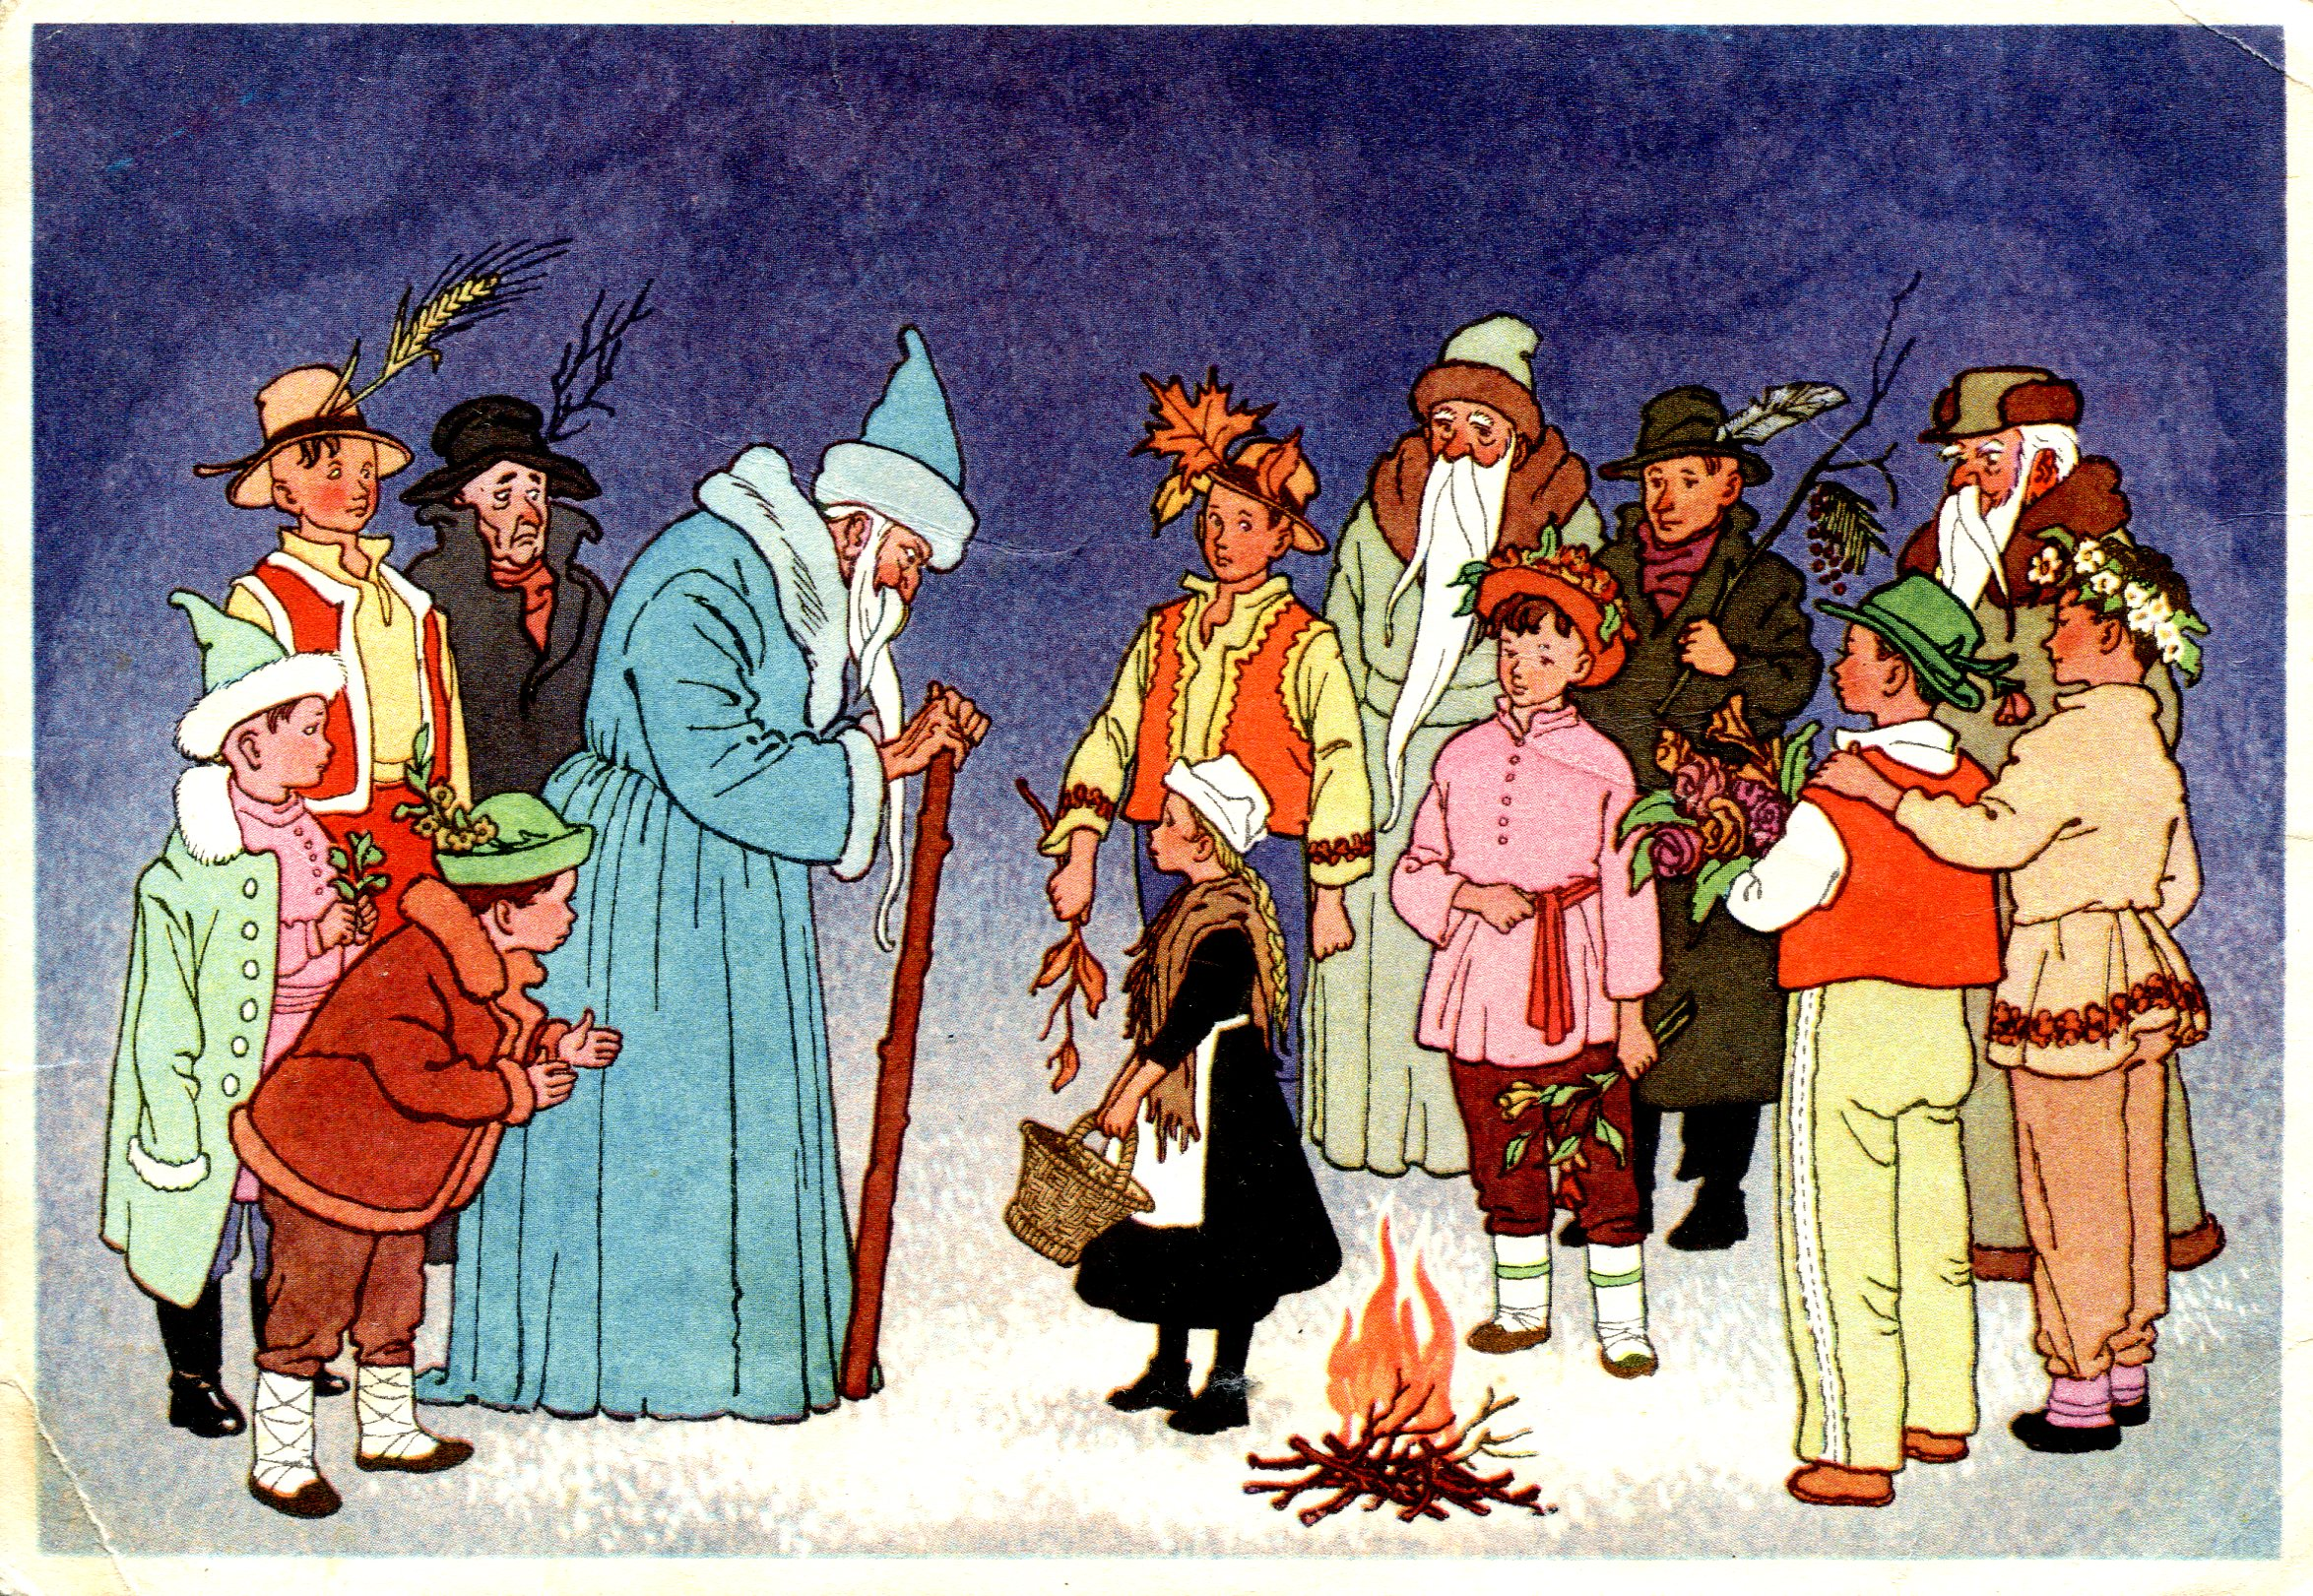
\includegraphics[width=0.8\linewidth]{12Months}
\end{figure}

12 Месяцев кружат свой небесный хоровод. Один за другим они занимают трон — от самого молодого и свирепого Января до пожилого и мудрого Декабря. Уходя, каждый Месяц громко выкрикивает цифру. За год из цифр складывается 12--значное число. Старый Год использует это число как щит на своём пути в Бездну Времени, защищаясь им от кошмарных созданий Вечности. От ударов щит разлетается на куски, соответствующие делителям числа.

Ваша задача~---~помочь Месяцам выковать для Старого Года щит, который нельзя было бы разбить на куски.

\subsection*{Формат входных данных}
В первой строке находится число уже ушедших Месяцев. Во второй~---~названные ими числа.

\subsection*{Формат выходных данных}
Вывести любое 12--значное число, начинающееся с заданных цифр и не имеющее нетривиальных делителей.
Гарантируется, что ответ есть. 


\subsection*{Примеры}

\texttt
{
	\begin{tabularx}{0.9\textwidth}{| X | X |}
       \hline
       \multicolumn{1}{|c|}{\inputFile} & \multicolumn{1}{c|}{\outputFile} \\ 
       \hline 
       \parbox[t]{\textheight}
       {
         5  \\
         64631 \\      
       } &
       646310554187 \\
       \hline
    \end{tabularx}
}

\newpage

\end{document}
